\documentclass{standalone}
\usepackage{tikz}
\usetikzlibrary{patterns, positioning}
\usepackage[sfdefault]{ClearSans} %% option 'sfdefault' activates Clear Sans as the default text font
\usepackage[T1]{fontenc}

\begin{document}
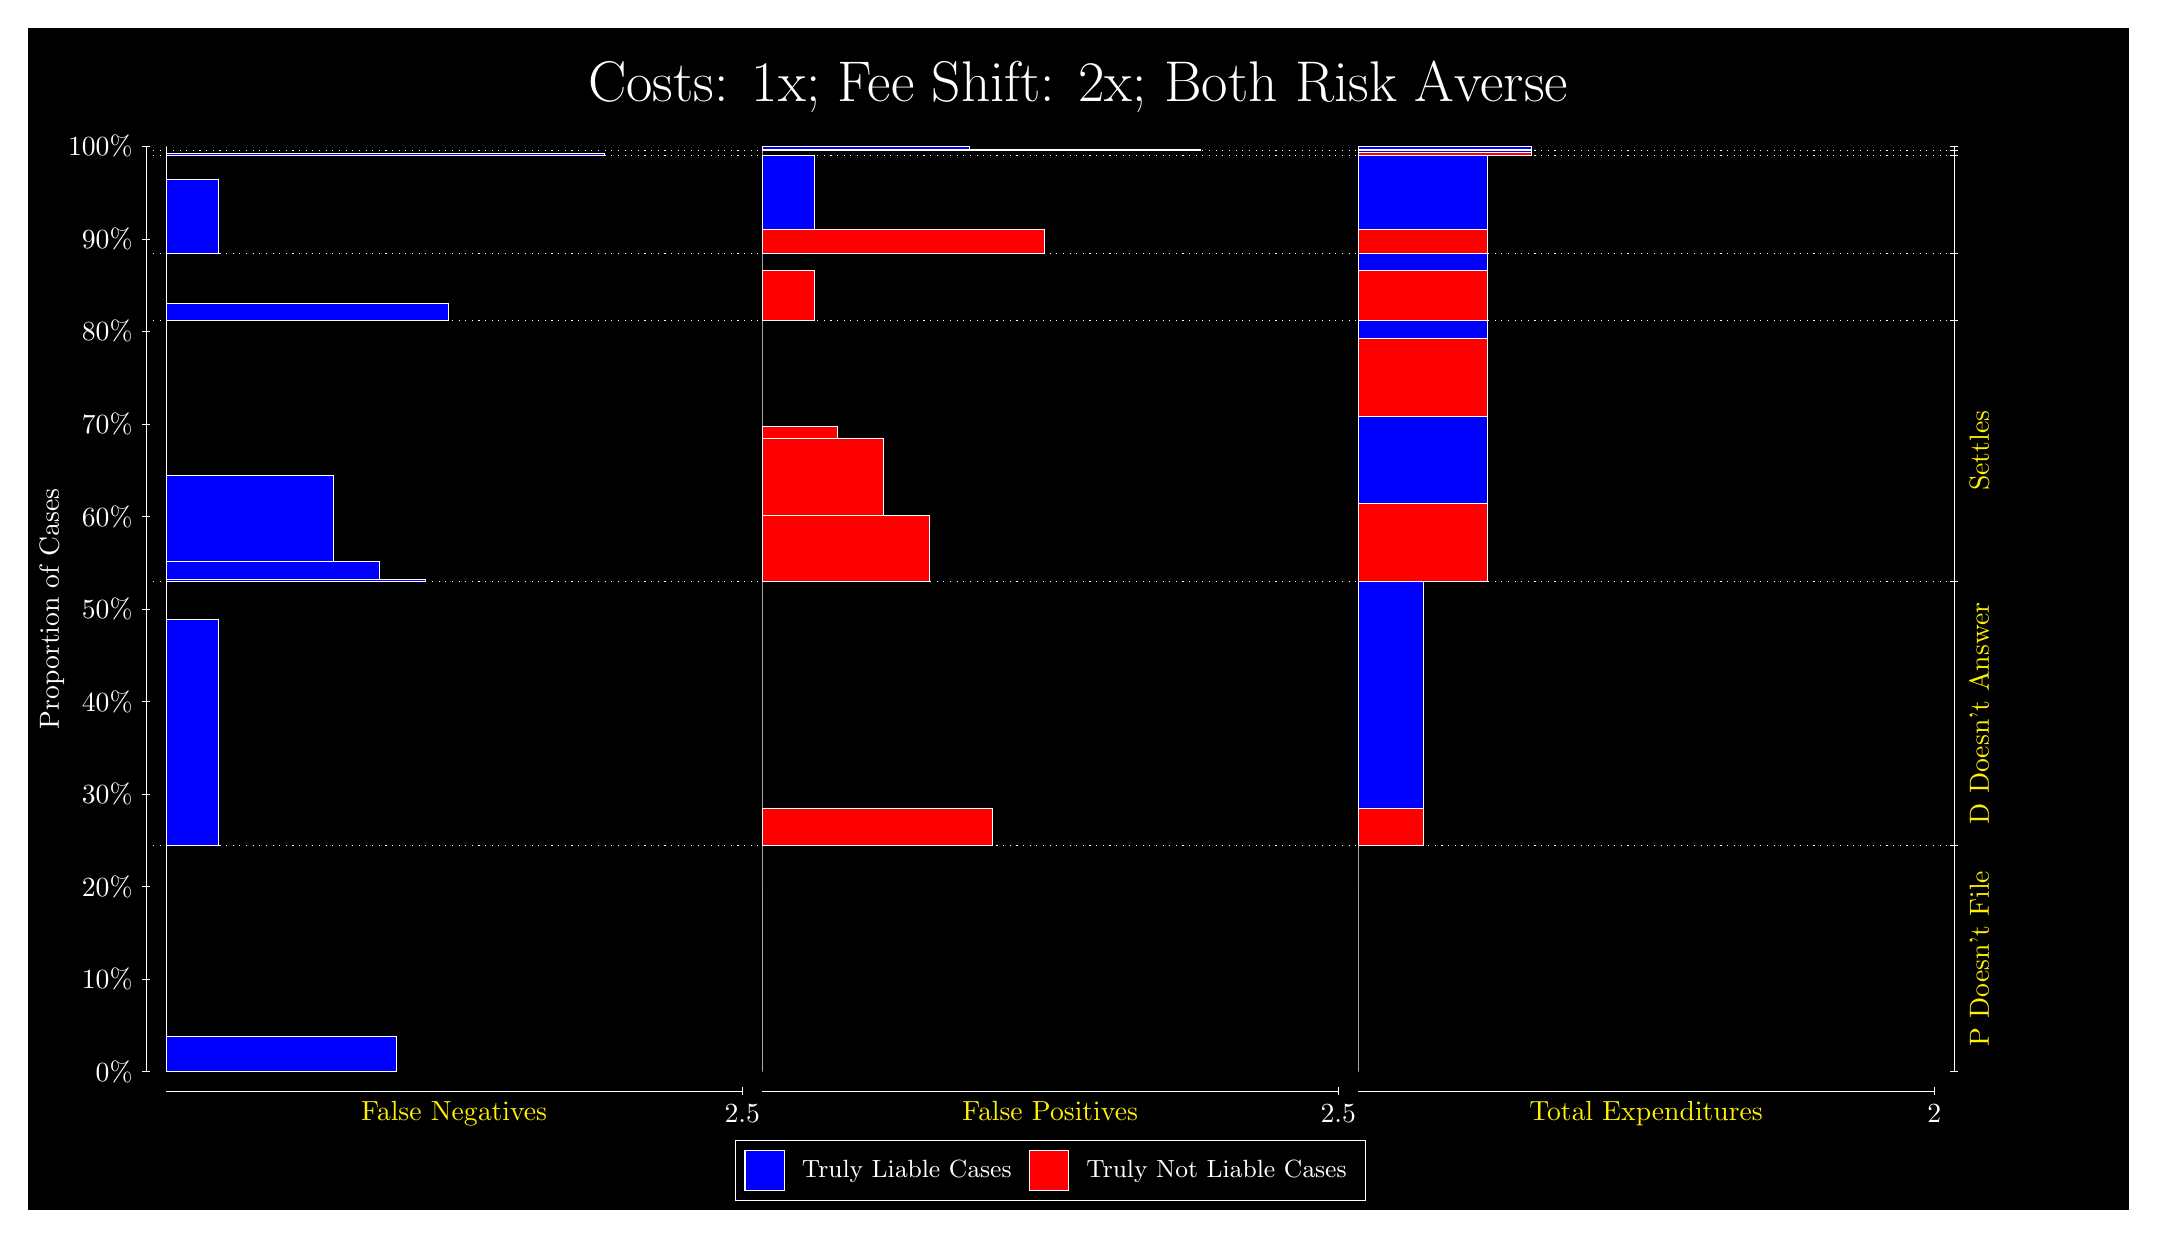
\begin{tikzpicture}
\draw[fill=black] (0,0) rectangle (26.667,15);
\draw[text=white] (0,13.5) rectangle (26.667,15) node[midway] {\huge Costs: 1x; Fee Shift: 2x; Both Risk Averse};
\draw[white, very thin] (1.5,1.75) -- (1.5,13.5);
\node[rotate=90, text=white, anchor=center] at (0.3, 7.625) {Proportion of Cases};
\draw[white, very thin] (1.45,1.75) -- (1.55,1.75);
\node[text=white, anchor=east] at (1.45, 1.75) {0\%};
\draw[white, very thin] (1.45,2.925) -- (1.55,2.925);
\node[text=white, anchor=east] at (1.45, 2.925) {10\%};
\draw[white, very thin] (1.45,4.1) -- (1.55,4.1);
\node[text=white, anchor=east] at (1.45, 4.1) {20\%};
\draw[white, very thin] (1.45,5.275) -- (1.55,5.275);
\node[text=white, anchor=east] at (1.45, 5.275) {30\%};
\draw[white, very thin] (1.45,6.45) -- (1.55,6.45);
\node[text=white, anchor=east] at (1.45, 6.45) {40\%};
\draw[white, very thin] (1.45,7.625) -- (1.55,7.625);
\node[text=white, anchor=east] at (1.45, 7.625) {50\%};
\draw[white, very thin] (1.45,8.8) -- (1.55,8.8);
\node[text=white, anchor=east] at (1.45, 8.8) {60\%};
\draw[white, very thin] (1.45,9.975) -- (1.55,9.975);
\node[text=white, anchor=east] at (1.45, 9.975) {70\%};
\draw[white, very thin] (1.45,11.15) -- (1.55,11.15);
\node[text=white, anchor=east] at (1.45, 11.15) {80\%};
\draw[white, very thin] (1.45,12.325) -- (1.55,12.325);
\node[text=white, anchor=east] at (1.45, 12.325) {90\%};
\draw[white, very thin] (1.45,13.5) -- (1.55,13.5);
\node[text=white, anchor=east] at (1.45, 13.5) {100\%};

\draw[white, very thin] (24.457,1.75) -- (24.457,13.5);
\draw[white, very thin] (24.407,1.75) -- (24.507,1.75);
\node[anchor=west] at (24.407, 1.75) {};
\draw[white, very thin] (24.407,4.6186) -- (24.507,4.6186);
\node[anchor=west] at (24.407, 4.6186) {};
\draw[white, very thin] (24.407,7.9782) -- (24.507,7.9782);
\node[anchor=west] at (24.407, 7.9782) {};
\draw[white, very thin] (24.407,11.291) -- (24.507,11.291);
\node[anchor=west] at (24.407, 11.291) {};
\draw[white, very thin] (24.407,12.141) -- (24.507,12.141);
\node[anchor=west] at (24.407, 12.141) {};
\draw[white, very thin] (24.407,13.389) -- (24.507,13.389);
\node[anchor=west] at (24.407, 13.389) {};
\draw[white, very thin] (24.407,13.447) -- (24.507,13.447);
\node[anchor=west] at (24.407, 13.447) {};
\draw[white, very thin] (24.407,13.5) -- (24.507,13.5);
\node[anchor=west] at (24.407, 13.5) {};

\draw[white, very thin, fill=blue] (1.75,1.75) rectangle (4.6775,2.1924);
\draw[white, very thin, fill=red] (1.75,2.1924) rectangle (1.75,4.6186);
\draw[white, very thin, fill=blue] (1.75,4.6186) rectangle (2.4087,7.4977);
\draw[white, very thin, fill=red] (1.75,7.4977) rectangle (1.75,7.9782);
\draw[white, very thin, fill=blue] (1.75,7.9782) rectangle (5.0435,7.9995);
\draw[white, very thin, fill=blue] (1.75,7.9995) rectangle (4.458,8.2343);
\draw[white, very thin, fill=blue] (1.75,8.2343) rectangle (3.8725,9.3218);
\draw[white, very thin, fill=red] (1.75,9.3218) rectangle (1.75,11.291);
\draw[white, very thin, fill=blue] (1.75,11.291) rectangle (5.3362,11.508);
\draw[white, very thin, fill=red] (1.75,11.508) rectangle (1.75,12.141);
\draw[white, very thin, fill=blue] (1.75,12.141) rectangle (2.4087,13.081);
\draw[white, very thin, fill=red] (1.75,13.081) rectangle (1.75,13.389);
\draw[white, very thin, fill=blue] (1.75,13.389) rectangle (7.3123,13.407);
\draw[white, very thin, fill=red] (1.75,13.407) rectangle (1.75,13.447);
\draw[white, very thin, fill=red] (1.75,13.447) rectangle (1.75,13.465);
\draw[white, very thin, fill=blue] (1.75,13.465) rectangle (1.75,13.5);
\draw[white, very thin, fill=red] (9.3189,1.75) rectangle (9.3189,4.1763);
\draw[white, very thin, fill=blue] (9.3189,4.1763) rectangle (9.3189,4.6186);
\draw[white, very thin, fill=red] (9.3189,4.6186) rectangle (12.246,5.0992);
\draw[white, very thin, fill=blue] (9.3189,5.0992) rectangle (9.3189,7.9782);
\draw[white, very thin, fill=red] (9.3189,7.9782) rectangle (11.441,8.8139);
\draw[white, very thin, fill=red] (9.3189,8.8139) rectangle (10.856,9.7936);
\draw[white, very thin, fill=red] (9.3189,9.7936) rectangle (10.27,9.947);
\draw[white, very thin, fill=blue] (9.3189,9.947) rectangle (9.3189,11.291);
\draw[white, very thin, fill=red] (9.3189,11.291) rectangle (9.9776,11.924);
\draw[white, very thin, fill=blue] (9.3189,11.924) rectangle (9.3189,12.141);
\draw[white, very thin, fill=red] (9.3189,12.141) rectangle (12.905,12.449);
\draw[white, very thin, fill=blue] (9.3189,12.449) rectangle (9.9776,13.389);
\draw[white, very thin, fill=red] (9.3189,13.389) rectangle (9.3189,13.43);
\draw[white, very thin, fill=blue] (9.3189,13.43) rectangle (9.3189,13.447);
\draw[white, very thin, fill=red] (9.3189,13.447) rectangle (14.881,13.465);
\draw[white, very thin, fill=blue] (9.3189,13.465) rectangle (11.954,13.5);
\draw[white, very thin, fill=red] (16.888,1.75) rectangle (16.888,4.1763);
\draw[white, very thin, fill=blue] (16.888,4.1763) rectangle (16.888,4.6186);
\draw[white, very thin, fill=red] (16.888,4.6186) rectangle (17.711,5.0992);
\draw[white, very thin, fill=blue] (16.888,5.0992) rectangle (17.711,7.9782);
\draw[white, very thin, fill=red] (16.888,7.9782) rectangle (18.534,8.9673);
\draw[white, very thin, fill=blue] (16.888,8.9673) rectangle (18.534,10.076);
\draw[white, very thin, fill=red] (16.888,10.076) rectangle (18.534,11.056);
\draw[white, very thin, fill=blue] (16.888,11.056) rectangle (18.534,11.291);
\draw[white, very thin, fill=red] (16.888,11.291) rectangle (18.534,11.924);
\draw[white, very thin, fill=blue] (16.888,11.924) rectangle (18.534,12.141);
\draw[white, very thin, fill=red] (16.888,12.141) rectangle (18.534,12.449);
\draw[white, very thin, fill=blue] (16.888,12.449) rectangle (18.534,13.389);
\draw[white, very thin, fill=red] (16.888,13.389) rectangle (19.083,13.43);
\draw[white, very thin, fill=blue] (16.888,13.43) rectangle (19.083,13.447);
\draw[white, very thin, fill=red] (16.888,13.447) rectangle (19.083,13.465);
\draw[white, very thin, fill=blue] (16.888,13.465) rectangle (19.083,13.5);
\draw[white, dotted] (1.5,4.6186) -- (24.457,4.6186);
\draw[white, dotted] (1.5,7.9782) -- (24.457,7.9782);
\draw[white, dotted] (1.5,11.291) -- (24.457,11.291);
\draw[white, dotted] (1.5,12.141) -- (24.457,12.141);
\draw[white, dotted] (1.5,13.389) -- (24.457,13.389);
\draw[white, dotted] (1.5,13.447) -- (24.457,13.447);
\draw[white, very thin] (1.75,1.5) -- (9.0689,1.5);
\node[text=yellow, anchor=north] at (5.4094, 1.5) {False Negatives};
\draw[white, very thin] (9.0689,1.45) -- (9.0689,1.55);
\node[text=white, anchor=north] at (9.0689, 1.45) {2.5};

\draw[white, very thin] (9.3189,1.5) -- (16.638,1.5);
\node[text=yellow, anchor=north] at (12.978, 1.5) {False Positives};
\draw[white, very thin] (16.638,1.45) -- (16.638,1.55);
\node[text=white, anchor=north] at (16.638, 1.45) {2.5};

\draw[white, very thin] (16.888,1.5) -- (24.207,1.5);
\node[text=yellow, anchor=north] at (20.547, 1.5) {Total Expenditures};
\draw[white, very thin] (24.207,1.45) -- (24.207,1.55);
\node[text=white, anchor=north] at (24.207, 1.45) {2};

\node[text=yellow, centered, rotate=90] at (24.777, 3.1843) {P Doesn't File};
\node[text=yellow, centered, rotate=90] at (24.777, 6.2984) {D Doesn't Answer};
\node[text=yellow, centered, rotate=90] at (24.777, 9.6344) {Settles};





\draw (12.978300999999998,1.5) node[draw=none] (baseCoordinate) {};
\begin{scope}[align=center]
        \matrix[scale=0.5, draw=white, below=0.5cm of baseCoordinate, nodes={draw}, column sep=0.1cm]{
            \node[rectangle, draw, minimum width=0.5cm, minimum height=0.5cm, fill=blue] {}; &
            \node[draw=none, font=\small, text=white] (B) {Truly Liable Cases}; &
            \node[rectangle, draw, minimum width=0.5cm, minimum height=0.5cm, fill=red] {}; &
            \node[draw=none, font=\small, text=white] (B) {Truly Not Liable Cases}; \\
            };
\end{scope}

\end{tikzpicture}
\end{document}